\chapter{Recomendação com similaridade semântica ponderada por links de recursos na DBPedia}
\label{cap:proposal}

\begin{quotation}[]{Steve Jobs}
You can't connect the dots looking forward; you can only connect them looking backwards. So you have to trust that the dots will somehow connect in your future.
\end{quotation}

Desde tempos o homem busca construir ferramentas e máquinas que ampliem e sustem sua capacidade de trabalho e produção. Com o advento dos programas de máquina, o \textit{software} tornou-se essencial para a demanda de problemas e desafios população. Como avaliado por \citep{Sommerville2010}, o software não se restringe a propriedades materiais das leis da física ou por processos de manufatura, o que por um lado simplifica a engenharia de software devido falta de restrições físicas, mas por outro, o torna complexo e custoso para mudanças. Assim, com a crescente quantidade e diversidade de computadores e dispositivos, é cada vez mais relevante a qualidade de software, visando a legibilidade, manutenção e evolução.

Neste capítulo serão apresentados os conceitos para a criação de sistema de recomendação com similaridade semântica ponderada por links de recursos na DBPedia\footnote{http://wiki.dbpedia.org}, sendo baseado nas preferências do usuário. Serão discutidas as tecnologias, arquiteturas, modelos dos dados, recomendação e algoritmos.

\section{Arquitetura}

Na arquitetura do sistema proposto, existe uma camada que é responsável pela construção das recomendações que possui os seguintes principais serviços:

\begin{itemize}
	\item{\textbf{Geração de Tokens}: Um dos objetivos do sistema é recomendar itens baseando-se no conteúdo não estruturado, no caso a sinopse dos filmes. A primeira tarefa é extrair as palavras, os \textit{tokens} relevantes dos textos, como nomes, adjetivos, lugares, entre outras, utilizando o processo de \ac{NLP}.}

	\item{\textbf{Cálculo da métrica de similaridade}: Após a geração das palavras importantes dos filmes, o sistema deve possuir um serviço para realizar o cálculo da similaridade entre dois tokens quaisquer, tirando proveito dos serviços da Web Semântica, no caso o DBPedia. Mais a frente será apresentada a equação da similaridade construída para este projeto, conforme consta na seção \ref{ssec:sim_rec}.}

	\item{\textbf{Geração das recomendações}: No último serviço, o sistema deverá construir um modelo dados através da geração de tokens para comparar as preferências do usuário com um filme, utilizando a métrica de similaridade proposta. Na seção \ref{sec:dataModel} é apresentado como é construído esses modelos e na seção \ref{ssec:sim_rec} o método utilizado para gerar a comparação e prover as recomendações.}
\end{itemize}

\section{Processo de Recomendação}

A proposta é criar uma recomendação baseada em conteúdo, ou seja, nos interesses que o usuário demonstrou no passado. A \textit{feature} analisada nos itens a serem avaliados, trata-se de um conteúdo não estruturado, no caso a descrição do item. Para este trabalho foi definido o domínio de filmes como exemplo de utilização, sendo assim, utilizando o texto da sinopse dos filmes como base para recomendação. A seguir será apresentado todas as etapas desde a captura dos dados até a apresentação das recomendações.

\begin{figure}
	\centering
	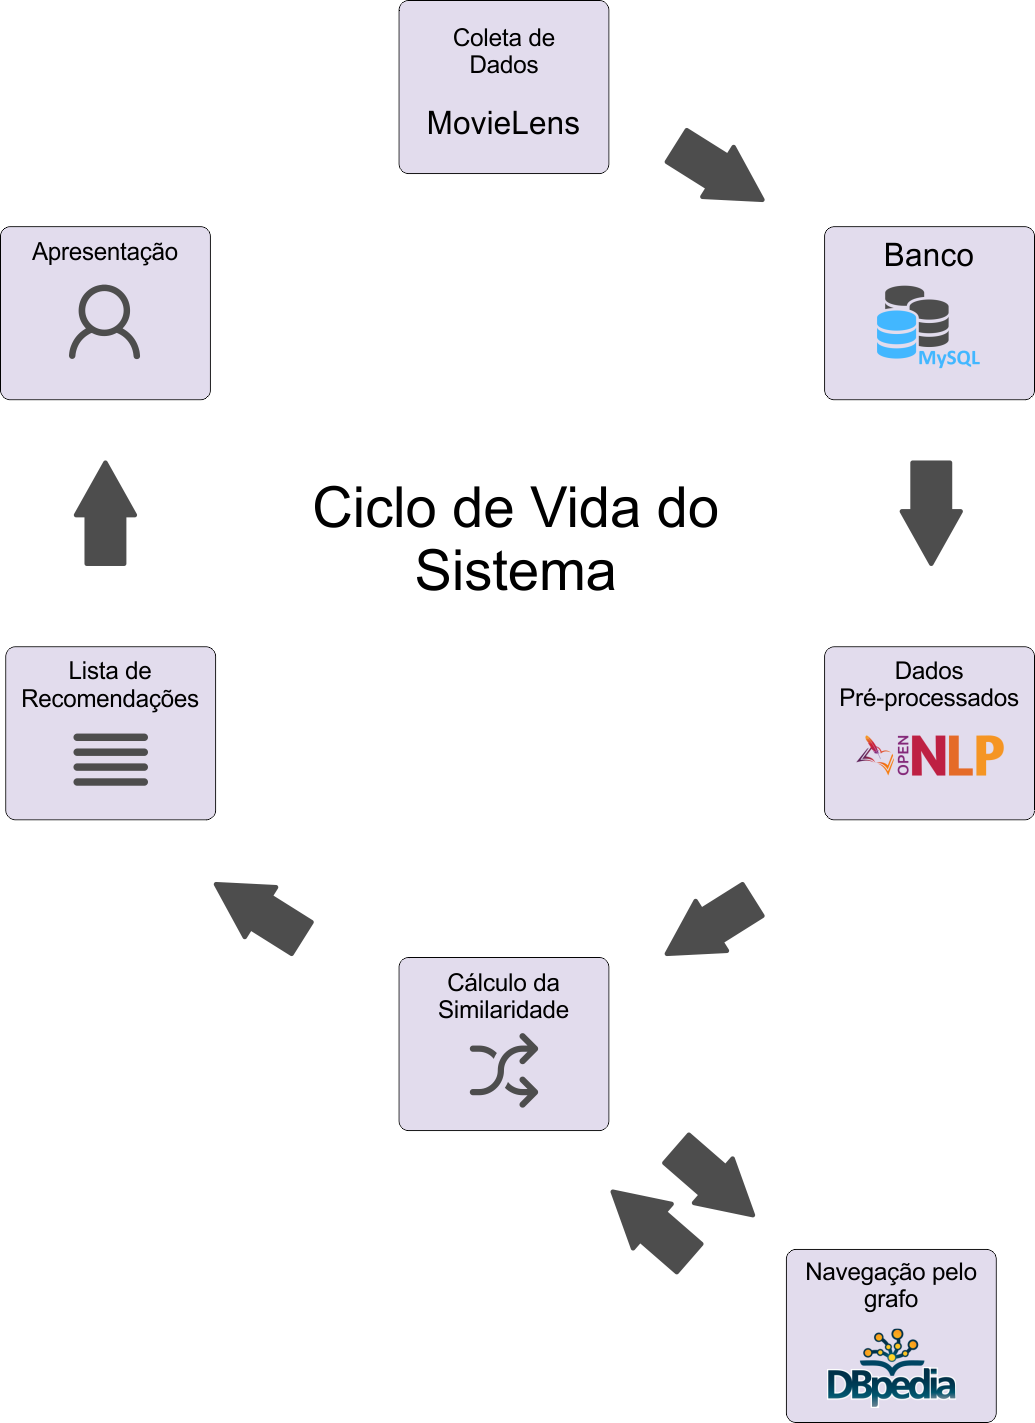
\includegraphics[scale=0.28]{imagens/recsys_fluxo.png}
	\caption{Fluxo das camadas do sistema de recomendação.}
	\label{fig:recsys_fluxo}
\end{figure}

\begin{enumerate}
	\item{\textbf{Coleta dos filmes}: Serão coletados dados dos filmes utilizando o projeto MovieLens\footnote{https://movielens.org} (ver \ref{sec:dataModel}).}
	
	\item{\textbf{Persistência dos dados}: Os dados coletados serão persistidos num banco de dados MySQL\footnote{https://www.mysql.com}.}

	\item{\textbf{Pré-processamento dos filmes}: Nessa etapa após a coleta dos filmes, os dados serão previamente processados para a geração de \textit{tokens} com \ac{NLP}, analisando a descrição dos itens (sinopse dos filmes). Após processados os \textit{tokens} serão persistidos no banco de dados.}

	\item{\textbf{Coleta das preferências do usuário}: Serão coletadas as avaliações dos usuários pelo projeto MovieLens, podendo assim montar um perfil de preferências.}

	\item{\textbf{Cálculo da Similaridade}: Após a etapa de pré-processamento dos filmes, será realizado o cálculo da similaridade entre os tokens do modelo do usuário e do filme, utilizando o métrica proposta \ac{RLWS}.}

	\item{\textbf{Geração das recomendações}: De posse do cálculo da similaridade, será gerado um conjunto de tamanho qualquer com os melhores \textit{scores} obtidos do cálculo desta similaridade. Posteriormente essa coleção filmes sugeridos será armazenada no banco, podendo ser atualizada conforme o perfil do usuário altera, ou novos filmes são cadastrados na base de dados. Na seção \ref{ssec:sim_rec} é demonstrado e discutido o algoritmo central para a similaridade e recomendação.}

	\item{\textbf{Apresentação dos resultados}: Por fim o sistema apresentará os resultados das recomendações para o usuário.}
\end{enumerate}

A Figura \ref{fig:recsys_fluxo} mostra como esse fluxo de funcionalidades é operado por todo o sistema. A seguir será o modelo dados elaborado para este trabalho.

\section{Modelo de dados}
\label{sec:dataModel}

Para a estrutura do sistema de recomendação foi elaborado um modelo de dados para o usuário, levando em conta suas preferências, além do modelo para as informações dos filmes. Nesta seção serão apresentados como os dados estão estruturados no banco de dados, além de estabelecer um modelo formal para o usuário e o filme, prontos para serem executado pelos camada de recomendação.

\subsection{Banco de dados}

Para trabalhar com as informações dos usuários e dos filmes, permitindo criar seus modelos para recomendação, os dados foram modelados e organizados de tal forma que possam ser facilmente persistidos e recuperados assim que necessário. A Figura \ref{fig:user_model} mostra como esses dados estão estruturados e interligados. É importante ressaltar algumas observações quanto a essa estrutura:

\begin{itemize}
	\item{A entidade \textit{rating} persiste as avaliações dos usuários, medidas de 0 a 5. Desta entidade será construída as preferências do usuário, ou seja, extraídos aqueles filmes que possuem boas avaliações refletindo aquilo que o usuário tem interesse.}

	\item{A entidade \textit{recomendation} persiste as sugestões de filmes calculadas pelo sistema, e o atributo \enquote{similarity} trata-se do algoritmo de similaridade utilizado, o que torna-se especialmente útil para realizar comparações com outros métodos (será discutido no \ref{cap:evaluation}).}

	\item{A entidade \textit{movie} persiste os dados dos filmes retirados do projeto MovieLens\footnote{https://movielens.org}, assim como o processamento da sinopse dos filmes para geração dos \textit{tokens}.}

	\item{A entidade \textit{idf} persiste o cálculo do \ac{IDF} da Equação \ref{eq:tfidf}, que servirá para o cálculo da similaridade cosseno, por motivos de comparação que serão discutidos no \ref{cap:evaluation}.}

	\item{As entidades \textit{lod\_cache} e \textit{lod\_cache\_relation} tratam-se do serviço de cache para o cálculo da similaridade, assim poupando tempo para consultas do serviço do DBPedia. Na seção \ref{sec:cache} a estrutura de cache dos sistema é melhor abordada.}
\end{itemize}

\begin{figure}
	\centering
	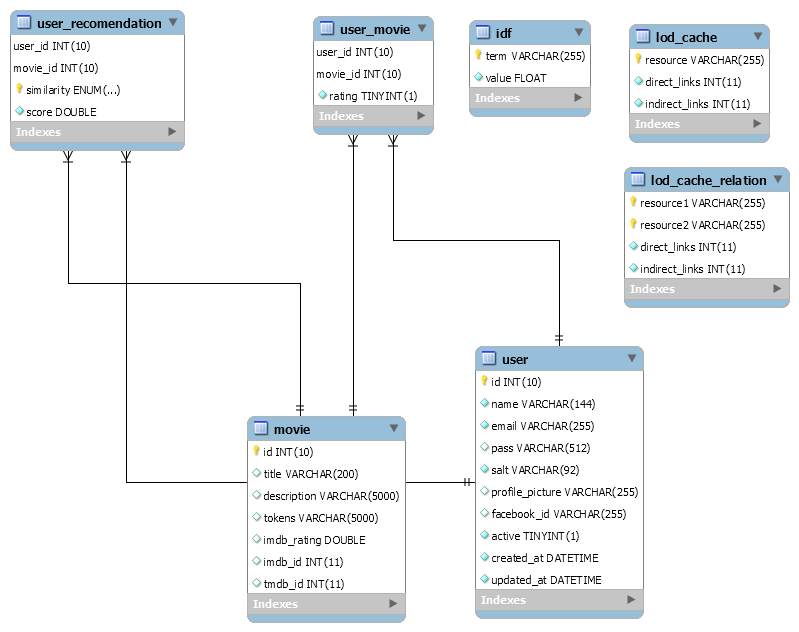
\includegraphics[scale=0.5]{imagens/user_model.png}
	\caption{Diagrama da modelagem dos dados extraído do banco MySQL}
	\label{fig:user_model}
\end{figure}

\label{ssec:database}
\subsection{Modelo de filmes}

Com a estrutura de dados utilizada para os filmes, é importante também formalizar como é seu modelo na recomendação, afinal este é o item a ser recomendado para o usuário. É definido um conjunto $X$ como sendo conjunto de todos os filmes, onde cada filme $F \subset X$ é um conjunto de tokens únicos $t_f$ extraídos pelo processo de \ac{NLP} (ver seção \ref{ssec:data_nlp}) através da sinopse deste. Para simplificar a formalização dos modelos, nota-se que o conjunto de termos $F$ do filme representa o filme junto com seus metadados, conforme definido em \ref{ssec:database}.

Desda forma formaliza-se o modelo de filmes conforme mostra as equações \ref{eq:film_model} e \ref{eq:film_model2}.

\begin{equation}
	X = \bigcup\limits_{i=1}^{\infty} F_{i}
\label{eq:film_model}
\end{equation}

\begin{equation}
	F = \{t_{f_1}, ..., t_{f_n} \; | \; 1 \leq n \leq \mathbb{N}^*\}
\label{eq:film_model2}
\end{equation}

\subsection{Modelo de usuários}
\label{ssec:user_model}

Os usuários inicialmente são estruturados como um conjunto de filmes, sendo extraídos aqueles bem avaliados por ele, à partir de uma nota de relevância $r$ baseada num modelo de cinco estrelas, onde nenhuma estrela é totalmente irrelevante e cinco totalmente relevante. Os filmes bem avaliados serão aqueles com relevância $r \geq 3,5$, portanto sendo suas preferências. Contudo, desta forma ainda não é possível realizar a comparação com o modelo de filmes utilizando a métrica de similaridade proposta (ver \ref{ssec:sim_rec}), devido a comparação ser de termo a termo. Uma opção inicial seria simplesmente calcular todos os termos dos filmes de preferência do usuário, utilizado no processo de \ac{NLP}, e uni-los num grande conjunto, porém isto tornaria o modelo de usuário muito custoso para ser utilizado, além de não escalar bem conforme as preferência do usuário aumentam. Sendo assim, optou-se por calcular os \enquote{melhores termos únicos} que representam o usuário, como sendo um conjunto de termos de um tamanho definido. Para calcular esses \enquote{melhores termos} é aplicado um modelo de frequência, o \ac{TFIDF} (ver Equação \ref{eq:tfidf}), que busca criar um ranking de termos determinando o quão importante são numa coleção, no caso a união de todos os conjuntos filmes e seus termos. Com isso é definido $Y$ como sendo o conjunto de todos os usuários $U$, e este por sua vez a união de todos os filmes $F_u$ e $P$ um subconjunto com aqueles de sua preferência, contendo todos os termos. Esses termos são denominados de termos do usuário, representado pelo elemento $t_u$. Assim como o modelo de filmes, os conjuntos $U$ e $P$ de termos do usuário também representa seus metadados. Posteriormente, define-se o conjunto $M_u$ sendo o \textbf{modelo do usuário} dos melhores termos $t_u \in P$, ao passarem pela seleção da função $M_{tfidf}$, que um define um subconjunto de um tamanho definido pela constante $z$. Por fim, o conjunto $Z$ é a união de todos os modelos de usuário $M_u$. O tamanho de $M_u$ será explorado no capítulo \ref{cap:evaluation}. As equações \ref{eq:user_model1} à \ref{eq:user_model5} formalizam a construção do modelo do usuário.


\begin{equation}
	Y = \bigcup\limits_{i=1}^{\infty} U_i \quad \text{ (todos os usuários)}
\label{eq:user_model1}
\end{equation}

\begin{equation}
	U = \bigcup\limits_{i=1}^{\infty} F_{u_i} \quad \text{ (todos os filmes do usuário)}
\label{eq:user_model2}
\end{equation}

\begin{equation}
	\begin{aligned}
		P = \bigcup\limits_{i=1}^{\infty} F_{u_i} \quad \{F_{u_i} \;|\; 3,5 \leq r \leq 5 \;\;\land\;\; r \in \mathbb{R} \;\;\land\;\; \frac{r}{0,5} \in \mathbb{N}\}\\
		\text{(todos os filmes de preferência do usuário)}
	\end{aligned}
\label{eq:user_model3}
\end{equation}

\begin{equation}
	\begin{aligned}
		(\forall t_u \in F_u \;\land\; F_u \subset P) \quad M_u = \{t_u \;| \; M_{tfidf}(P, z), \; |M_u| = z \; \land \; z \in \mathbb{N}^*\} \\
		\text{ (aplicação dos melhores termos do usuário)}
	\end{aligned}
\end{equation}

\begin{equation}
	Z = \bigcup\limits_{i=1}^{\infty} M_{u_i} \quad \text{ (todos os modelos de usuários)}
\label{eq:user_model5}
\end{equation}

\subsection{Preparação dos dados para recomendação}
\label{ssec:data_nlp}

Antes da execução das recomendações é necessário realizar a etapa do pré-processamento dos dados. Para cada filme são gerados \textit{tokens} que são palavras relevantes presentes na descrição. Essas palavras relevantes tratam-se do processo de exclusão daquelas que pouco agregam significado ao que se refere a temática do filme, como é o exemplo de preposições, conjunções e artigos.

Para extração dessas palavras, foi utilizado o processo denominado de \ac{NLP} que envolve uma série de tarefas para o processamento de linguagens naturais \footnote{Linguagem desenvolvida naturalmente pelo ser humano de forma não premeditada, no caso a escrita}, para compreensão e interação entre máquinas e humanos, conforme é apresentado por \cite{Collobert:2011}. A Figura \ref{fig:nlp} ilustra as tarefas comuns no processamento de linguagem natural. O foco é extrair dos termos palavras com fortes significados, como adjetivos, verbos, além de também identificar substantivos, inclusive os compostos. Abaixo consta as tarefas que foram utilizadas para no processo de preparação dos dados:

\begin{itemize}
	\item{\textbf{Tokenization}: Esta tarefa consiste em segmentar um texto em partes da linguagem, sendo responsável por criar separar em tokens. Muitas vezes também é utilizado o processo de \textit{chunking} que visa ir além de separar as palavras mas segmentar o texto em frases em partes maiores do texto, algo que não foi utilizado neste projeto.}
	\item{\textbf{Tagging, \ac{POS}}: O objetivo desta tarefa é reconhecer as palavras do processo de tokenization como "partes do discurso", criando \textit{tags} para identificar o que elas representam na linguagem. Nesta parte é onde se classificam as palavras em verbos, adjetivos, substantivos, pontuações etc.}
	\item{\textbf{\ac{NER}}: Esta tarefa objetiva reconhecer nas palavras e tokens aquelas que tratam-se de nomes próprios, além de associá-las à algum tipo, como pessoas, lugares, moedas etc.}
\end{itemize}

\begin{figure}
	\centering
	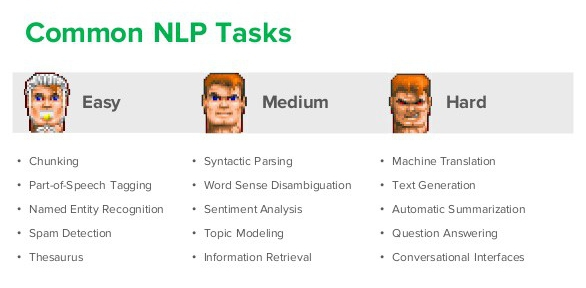
\includegraphics[scale=0.70]{imagens/nlp.jpg}
	\caption{Segmentação de tarefas no NLP. \citep{NLP2016}}
	\label{fig:nlp}
\end{figure}

Para facilitar a execução dessas tarefas do \ac{NLP}, optou-se por utilizar o \textit{framework} OpenNLP\footnote{https://opennlp.apache.org}, conforme também abordado na seção \ref{ssec:open_nlp}, que através de um modelo de treinamento, possibilita facilmente realizar o processo de \textit{tagging}, identificando as partes do discurso. Uma vez realizada a anotação do texto definiu-se apenas capturar as palavras marcadas com as \textit{tags} conforme mostra a tabela \ref{tab:nlp_tags}. Vale ressaltar que essas definições foram concebidas para língua inglesa, uma vez que as sinopses importadas do projeto MovieLens\footnote{https://movielens.org} estão nessa língua.

Em seguida é incluído ao conjunto de termos os tokens da tarefa \ac{NER}, o que não é meramente o reconhecimento de nomes próprios do texto, mas também de nomes compostos. Esse processo é de grande valia para a etapa de similaridade uma vez que tendo um nome como "Buzz Lightyear", apenas utilizando o processo da marcação das partes do discurso, resultaria em dois termos "Buzz" e "Lightyear", sendo que o ideal seja também ter o nome composto por inteiro. Os substantivos próprios obtidos pelo processo \ac{POS} também são mantidos no conjunto de termos, uma vez que o framework utilizado no processo de \ac{NLP} apenas extrai, nomes, lugares e organizações. Para os nomes reconhecidos nesse processo também foi realizada uma formatação para adequação à consultas \ac{SPARQL}, ou seja, nomes compostos como "Buzz Lightyear" são formatados para "Buzz\textunderscore Lightyear", mantendo as iniciais maiúsculas e separando as palavras por "\textunderscore" . A tabela \ref{tab:nlp_example} demonstra alguns exemplos do tratamento da descrição de filmes para geração de \textit{tokens}.

\begin{table}[H]
	\centering
	\caption{Relação das tags das partes do discurso}
	\def\arraystretch{1.3} % padding da linhas da tabela
	\begin{tabular}{| m{1.3cm} | m{9.4cm}| c | m{2cm}}
		\hline
		\multicolumn{1}{|c|}{\bfseries Tag} & \multicolumn{1}{c|}{\bfseries Descrição} \\ \hline
		NN & Substantivo comum, singular ou incontável \\ \hline
		NNS	& Substantivo comum, plural \\ \hline
		NNP	& Substantivo próprio, singular \\ \hline
		NNPS & Substantivo próprio, plural \\ \hline
		JJ & Adjetivo \\ \hline
		JJR & Adjetivo comparativo \\ \hline
		JJS & Adjetivo superlativo \\ \hline
		FW & Palavra estrangeira \\ \hline
		VB & Verbo, forma base \\ \hline
	\end{tabular}
\label{tab:nlp_tags}
\end{table}

\begin{table}[H]
	\centering
	\caption{Exemplos da geração de tokens}
	\def\arraystretch{1.3} % padding da linhas da tabela
	\begin{tabular}{|p{2cm}|p{6cm}|p{6cm}|}
	\hline
	\textbf{Filme} & \textbf{Sinopse} & \textbf{Tokens} \\ \hline
	Toy Story & Led by Woody, Andy's toys live happily in his room until Andy's birthday brings Buzz Lightyear onto the scene. Afraid of losing his place in Andy's heart, Woody plots against Buzz. But when circumstances separate Buzz and Woody from their owner, the duo eventually learns to put aside their differences.& Woody, Andy, Toys, Room, Andy, Birthday, Scene, Place, Andy, Heart, Woody, Plots, Circumstances, Woody, Owner, Duo, Put, Differences, Buzz\_Lightyear \\ \hline
	GoldenEye & James Bond must unmask the mysterious head of the Janus Syndicate and prevent the leader from utilizing the GoldenEye weapons system to inflict devastating revenge on Britain. & Unmask, Mysterious, Head, Janus, Syndicate, Prevent, Leader, Goldeneye, Weapons, System, Inflict, Devastating, Revenge, Britain, James\_Bond \\ \hline
	\end{tabular}
\label{tab:nlp_example}
\end{table}

\section{Modelo de Recomendação}
\label{ssec:sim_rec}

A criação de um modelo de recomendação envolve sugerir novos itens, sendo caracterizada como uma predição de o quão provável o usuário terá interesse no conteúdo recomendado. Nesta seção serão apresentadas as etapas que existem para construção deste modelo, que envolve a definição da métrica de similaridade, através da equação da similaridade semântica (ver \ref{ssec:formula_rlws}) e da construção da recomendação (ver \ref{ssec:rec_alg}).

Conforme abordado no capítulo \ref{cap:semantic_web}, a similaridade semântica utiliza e retira proveito das estruturas de uma ontologia que neste caso trata-se das acessíveis através do DBPedia\footnote{http://wiki.dbpedia.org}. Cada termo de um filme será considerado como um potencial recurso na DBPedia, e os recursos tratam-se de entidades de ontologias mapeadas no grafo dos princípios do \ac{LOD}. Diante disso, a métrica proposta é estabelecer uma equação de similaridade, utilizando-se de um modelo que considera a estrutura desses recursos, analisando a quantidade de relações e links diretos ou indiretos entre tais recursos. 

Para estabelecer a equação proposta, considerou-se dois trabalhos relacionados com similaridade semântica, o de \cite{PassantLDSD} que apresenta a equação \ac{LDSD}, e mais recentemente de \cite{PiaoResim}, que propõem o \ac{RESIM}. O primeiro trabalho tenta estabelecer a importância que um recurso tem em relação ao total de relações da união de dois recursos, sem preferências entre links diretos e indiretos, enquanto que \cite{PiaoResim} estende e modifica esse entendimento criando uma média ponderada entre as relações dos recursos e a similaridade entre suas propriedades.

Este trabalho propõe então um novo método denominado de \ac{RLWS}, para realizar a medida da similaridade entre dois recursos presentes no DBPedia, criando uma média ponderada entre a relevância dos links diretos e indiretos, para gerar um valor na escala de 0 a 1, onde valores menores denotam menor similaridade. Além disso é apresentado o modelo de recomendação construindo uma similaridade entre um modelo que represente o usuário e suas preferências, com o modelo do filme. 

Para esse modelo de recomendação foi concebida uma razão de similariade inspirada em modelos mais complexos como o \ac{WMD}, introduzido por \cite{WMD:2015}, que define um método para calcular distância entre documentos utilizando um cálculo de distância entre palavras baseado no \textit{word2vec} desenvolvido pelo Google\footnote{https://google.com} \citep{word2vec:2013}. O método \ac{WMD} estabelece um peso de cada palavra num documento e o "custo de transformação" dela em relação às outras palavras do documento a ser comparado, obtendo-se como a distância o melhor fluxo para essa "transformação"\;, algo análogo ao problema do transporte \citep{Transporte:2016}. Na proposta deste trabalho não será utilizada uma distância entre palavras e sim uma simlariadade com \ac{RLWS}, além não ter uma distãncia entre documentos (no caso entre o modelo do filme e do usuário) que leve em consideração peso de palavras, realizando então um cálculo de média simplificado.

\subsection{Equação para similaridade semântica}
\label{ssec:formula_rlws}

A Equação \ref{eq:rlws} demonstra o cálculo da similaridade semântica, que consiste em um conjunto de 5 funções  $C_d$, $C_i$, $C_{di}$, $C_{do}$, $C_{io}$. Estas funções tratam-se de levar em consideração a quantidade links de um recurso ou entre recursos dentro de um conjunto seguindo os princípios do \ac{LOD}, de acordo com a seguinte definição \citep{PiaoResim}:

\begin{definition}
Um conjunto que segue os princípios LOD é um grafo $G$ tal que $G = (R, L, I)$ aonde $R = \left\{r_1, r_2, ..., r_n\right\}$ é um conjunto de recursos identificados por suas URI, $L = \left\{i_1, i_2, ..., i_n\right\}$ é um conjunto de instâncias desses links entre recursos, como $i_i = <l_j, r_a, r_b>$.
\end{definition}

\begin{equation}
	RLWS(r_a, r_b) =
	\begin{dcases*}
		1 \text{,} \;\; URI(r_a) = URI(r_b) \;\; \text{ou} \;\; r_a \; \textit{ dbo:wikiPageRedirects } \; r_b\\
		\frac{S_d(r_a, r_b) * w_d + S_i(r_a, r_b) * w_i}{w_d + w_i}, \; \text{caso contrário}
	\end{dcases*}
\label{eq:rlws}
\end{equation}

\begin{equation}
	S_d(r_a, r_b) = 1 - \frac{1}{1 + \frac{\sum_i C_{di}(l_i, r_a, r_b) + \sum_i C_{do}(l_i, r_a, r_b)}{1 + \log (C_d(r_a) + C_d(r_b))}}
\label{eq:rlws_ex1}
\end{equation}

\begin{equation}
	S_i(r_a, r_b) = 1 - \frac{1}{1 + \frac{\sum_i C_{ii}(l_i, r_a, r_b)}{1 + \log (C_i(r_a) + C_i(r_b))}}
\label{eq:rlws_ex2}
\end{equation}

A equação possui um condicional que implica o valor 1 quando dois recursos comparados tenham a mesma \textit{URI} ou estejam relacionados pela propriedade \textit{dbo:wikiPageRedirects}. Essa propriedade nada mais trata de redirecionamentos do próprio serviço do DBPedia, que quando consultando recursos como "Movie" e "Film", resultam na mesma página, pois são redirecionamentos. Para maior generalização o termo "link" será utilizado para se referir tanto a ligações como recursos ou propriedades relacionadas. As funções $C_d$ e $C_i$ tratam-se de computar os links distintos de um recurso qualquer, ou seja todas as ligações distintas a outros recursos, de forma direta e indireta respectivamente. No caso da função $C_d$, são computados todos os recursos distintos que sejam alcançados por uma propriedade qualquer através de um recurso analisado em questão, mais aqueles que partem de outro recurso e chegam nesse mesmo desejado. O exemplo da Figura \ref{fig:cd_links} apresenta o recurso "Tom\_Cruise" a ser calculado, que possui um link direto sainte para o recurso "American\_film\_producers" através da propriedade "sujeito de", e outro link direto de entrada pelo recurso "Jack\_Reacher" através da propriedade "retratado por".

\begin{figure}
	\centering
	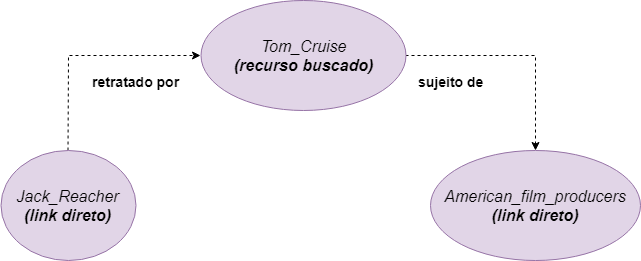
\includegraphics[scale=0.35]{imagens/cd_links.png}
	\caption{Imagem que retrata os links diretos saintes e entrantes de um recurso.}
	\label{fig:cd_links}
\end{figure}

A contagem desses links é realizada através da consulta \ac{SPARQL} conforme a Figura \ref{fig:cd_links}. Alguns filtros de propriedades são realizados, pois não são relevantes para a consulta. A propriedade \textit{dbo:wikiPageRedirect} é realizada por outra consulta a parte, mas é adicionada no filtro, para não levá-la em consideração durante a contagem. Para a função $C_i$ apenas são contabilizados os links indiretos de saída, por motivos de desempenho de consultas SPARQL no DBPedia. A imagem \ref{fig:ci_links} retrata o cenário para os links indiretos, e o Código \ref{cod:sparql_ci} a contagem dos links indiretos. Quanto para as funções $C_{di}$, $C_{do}$ e $C_{io}$, referem-se a contagem dos links distintos compartilhados entre dois recursos, sendo os dois primeiros de forma direta e o último de forma indireta. Os Códigos \ref{cod:sparql_cdio} e \ref{cod:sparql_cio} apresentam as consultas \ac{SPARQL} para realizar a contagem dos links.

\begin{lstlisting}[caption=Consulta SPARQL para contagem de links diretos, language=SQL, frame=single, label={cod:sparql_cd}, float, numbers=left]
PREFIX  :  <http://dbpedia.org/resource/>
PREFIX  dbo:  <http://dbpedia.org/ontology/>
SELECT (count (distinct ?p1) as ?x)
WHERE {
	{values (?r1) {(<http://dbpedia.org/resource/r1>)} ?r1 ?p1 ?r2 . FILTER (?r1 != ?r2)}
	UNION
	{values (?r1) {(<http://dbpedia.org/resource/r1>)} ?r2 ?p1 ?r1 . FILTER (?r1 != ?r2)}
	FILTER ( ?p1 != dbo:wikiPageID )
	FILTER ( ?p1 != dbo:wikiPageRevisionID )
	FILTER ( ?p1 != dbo:wikiPageRedirects )
	FILTER ( ?p1 != dbo:wikiPageExternalLink )
	FILTER ( ! isLiteral(?r2) )
}
\end{lstlisting}

O objetivo da equação é obter o quão relevante é o relacionamento entre dois recursos em relação a soma dos relacionamentos deles a quaisquer outros, obtendo $S_d$ para uma "similaridade direta" entre $r_a$ e $r_b$, e $S_i$ para uma "similaridade indireta". Posteriormente essas similaridades são aplicada na média ponderada com os pesos $w_d$ e $w_i$, obtendo esta similaridade semântica média com o peso dos links. É importante ressaltar que para manter a equação correta é necessário que a soma dos pesos seja igual 1. A introdução das funções de $\log$ tem o objetivo de transformar os dados, suavizando o enviesamento da proporção entre os valores do total da soma de links diretos em relação aos links da comparação de $r_a$ e $r_b$. De caráter ilustrativo, quando comparamos termos como "United\_States" e "Group" em relação aos links indiretos, tem uma soma de 429.116 links que em comparação entre o que relaciona um ao outro é de 2.010.

\begin{figure}
	\centering
	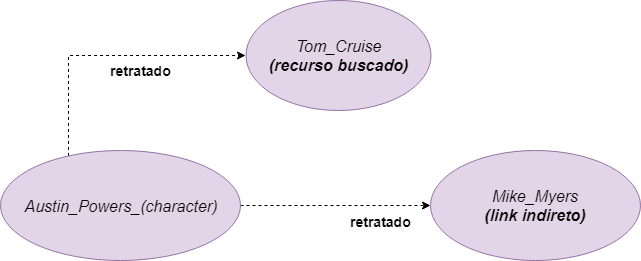
\includegraphics[scale=0.35]{imagens/ci_links.png}
	\caption{Imagem que retrata os links indiretos saintes de um recurso.}
	\label{fig:ci_links}
\end{figure}

\begin{lstlisting}[caption=Consulta SPARQL para contagem de links indiretos., language=SQL, frame=single, label={cod:sparql_ci}, float, numbers=left]
PREFIX  :  <http://dbpedia.org/resource/>
PREFIX  dbo:  <http://dbpedia.org/ontology/>
SELECT (count (distinct ?r2) as ?x)
WHERE {
	{values (?r1) {(<http://dbpedia.org/resource/r1>)} ?r2 ?p1 ?r1 . ?r2 ?p2 ?r3 . FILTER (?r1 != ?r3 && ?r2 != ?r1 && ?r2 != ?r3)}
	FILTER ( ?p1 != dbo:wikiPageID )
	FILTER ( ?p1 != dbo:wikiPageRevisionID )
	FILTER ( ?p1 != dbo:wikiPageRedirects )
	FILTER ( ?p1 != dbo:wikiPageExternalLink )
	FILTER ( ! isLiteral(?r2) )
	FILTER ( ?p2 != dbo:wikiPageID )
	FILTER ( ?p2 != dbo:wikiPageRevisionID )
	FILTER ( ?p2 != dbo:wikiPageRedirects )
	FILTER ( ?p2 != dbo:wikiPageExternalLink )
}
\end{lstlisting}

\begin{lstlisting}[caption=Consulta SPARQL para contagem de links diretos (saíntes e entrantes) entre dois recursos., language=SQL, frame=single, label={cod:sparql_cdio}, float, numbers=left]
PREFIX  :  <http://dbpedia.org/resource/>
PREFIX  dbo:  <http://dbpedia.org/ontology/>
SELECT (count(distinct ?p1) as ?x)
WHERE {
	{values (?r1 ?r2) {(<http://dbpedia.org/resource/r1> <http://dbpedia.org/resource/France>)} ?r1 ?p1 ?r2 . FILTER (?r1 != ?r2) }
	UNION
	{values (?r1 ?r2) {(<http://dbpedia.org/resource/r2> <http://dbpedia.org/resource/Paris>)} ?r1 ?p1 ?r2 . FILTER (?r1 != ?r2) }
	FILTER ( ?p1 != dbo:wikiPageID )
	FILTER ( ?p1 != dbo:wikiPageRevisionID )
	FILTER ( ?p1 != dbo:wikiPageRedirects )
	FILTER ( ?p1 != dbo:wikiPageExternalLink )
	FILTER ( ! isLiteral(?r2) )
}
\end{lstlisting}

\begin{lstlisting}[caption=Consulta SPARQL para contagem de links indiretos (saíntes) entre dois recursos., language=SQL, frame=single, label={cod:sparql_cio}, float, numbers=left]
PREFIX  :  <http://dbpedia.org/resource/>
PREFIX  dbo:  <http://dbpedia.org/ontology/>
SELECT (count (distinct ?r2) as ?x)
WHERE {
	{values (?r1 ?r3) {(<http://dbpedia.org/resource/r1> <http://dbpedia.org/resource/r2>)} ?r2 ?p1 ?r1 . ?r2 ?p2 ?r3 . FILTER (?r1 != ?r3 && ?r2 != ?r1 && ?r2 != ?r3)}
	FILTER ( ?p1 != dbo:wikiPageID )
	FILTER ( ?p1 != dbo:wikiPageRevisionID )
	FILTER ( ?p1 != dbo:wikiPageRedirects )
	FILTER ( ?p1 != dbo:wikiPageExternalLink )
	FILTER ( ! isLiteral(?r2) )
	FILTER ( ?p2 != dbo:wikiPageID )
	FILTER ( ?p2 != dbo:wikiPageRevisionID )
	FILTER ( ?p2 != dbo:wikiPageRedirects )
	FILTER ( ?p2 != dbo:wikiPageExternalLink )
}
\end{lstlisting}

Por último é destacável notar que a equação exibe os axiomas abaixo que são importantes para a consistência da similaridade:

\begin{itemize}
	\item{\textbf{Similaridade reflexiva}: $RLWS(r_a, r_a) = RLWS(r_b, r_b), \text{ para todo } r_a \text{ e } r_b$.}
	\item{\textbf{Simetria}: $RLWS(r_a, r_b) = RLWS(r_b, r_a), \text{ para todo } r_a \text{ e } r_b$.}
\end{itemize}

\subsection{Algoritmo da recomendação}
\label{ssec:rec_alg}

Com equação de similaridade semântica entre dois recursos é possível comparar os termos dos filmes que por sua vez habilita a construção de um \textit{ranking} de filmes mais similares em relação as preferências do usuário. Para montar esse perfil de preferências, conforme foi apresentado na seção \ref{ssec:user_model}, o usuário se tornará um conjunto de termos, podendo ser interpretado como uma \textit{query}, no mesmo formato do modelo de filmes, onde objetivo é uma comparação entre um conjunto e outro, utilizando a similaridade proposta. Apesar de ser possível utilizar todos os termos de todos os filmes que o usuário gostou, optou-se por escolher uma quantidade determinada de "melhores termos únicos". Esses melhores termos são calculados através de um modelo construído pela frequência, o \ac{TFIDF}. Esse cálculo trata-se de uma estatística que tem por objetivo de refletir o quão importante um termo é para o documento numa coleção \citep{rajaraman_ullman_2011}.

A Equação \ref{eq:tf}, trata-se da frequência do termo em relação ao documento, o que neste caso refere-se a cada termo de um filme do usuário e sua frequência em relação aos termos desse filme. Quanto a segunda, \ref{eq:idf}, refere-se ao inverso da frequência do documento, que busca balancear os termos muito frequentes em relação aos pouco frequentes, uma vez que não necessariamente todos os termos tem importância igual. Dessa forma é construída um conjunto de termos únicos de todos os filmes do usuário que para cada um deles seja contabilizado a presença na coleção dos filmes. Por fim, cada termo recebe um \textit{score}, conforme a Equação {\ref{eq:tfidf}}.

\begin{equation}
	TFIDF(t) = TF(t) * IDF(t)
\label{eq:tfidf}
\end{equation}

\begin{equation}
	TF(t) = \frac{f_{t,d}}{f_{t',d} : t' \in d}
\label{eq:tf}
\end{equation}

\begin{equation}
	IDF(t) = \log (\frac{N}{d \in D : t \in d})
\label{eq:idf}
\end{equation}

Com a equação pronta basta estabelecer um \textit{ranking} de termos, escolhendo aqueles com os melhores \textit{scores}, para montar o perfil do usuário. Nota-se que com esta equação obtém-se um score por termo de cada filme, e eventualmente este termo pode reaparecer em outro conjunto de termos de outro filme, possuindo um score diferente. Entretanto, como é estabelecido um ranking de melhores termos únicos, não há interesse na presença de dois termos iguais com scores diferentes, o interesse é montar um perfil com termos distintos e variados com melhor pontuação. Vale ressaltar que conforme estabelecido em \ref{ssec:user_model} é definida uma constante $z$ como sendo o tamanho do conjunto desses \enquote{melhores termos} extraídos desse ranking criado. No capítulo \ref{cap:evaluation} o impacto do tamanho do perfil do usuário será melhor explorado.  Sendo assim, é definida a Equação \ref{eq:max_tfidf}, como extensão para obtenção dos melhores termos, que avalia cada termo único $t$ do modelo de usuário $M_u$, escolhendo aqueles com melhor score.

\begin{equation}
	M_u(t) = max \; TFIDF(t)
\label{eq:max_tfidf}
\end{equation}

Definido o conjunto de termos do usuário, este será comparado com o conjunto de termos de todos os filmes que o usuário não tenha informado preferência, ou seja, que ele desconheça, denominado de $D_u$, pois o objetivo é recomendar novos itens. Para melhor compreensão o conjunto dos termos do filme $F$ e do usuário $U$, representam respectivamente seus metadados, conforme estabelecido em \ref{ssec:database}. Sendo assim, almeja-se obter os filmes com os melhores \textit{scores} de recomendação, definido por $R_{max, U}$, que é o resultado da maximização das melhores recomendações $R$ obtida pela equação função $S(M_u, F)$, cuja fornece a similaridade entre o modelo de usuário e o filme. As equações abaixo demonstram a formalização do cálculo da recomendação:

\begin{equation}
	D_u = X - U \quad \text{(filmes que o usuário desconhece)}
\label{eq:rec_model_movies}
\end{equation}

\begin{equation}
	\begin{aligned}
		(\forall t_u \in M_u \;\land\; \forall t_f \in F) \quad recModel(U, F) = M_u \times F\\
		= \{\{t_{u_1}, t_{f_1}\}, \{t_{u_1}, t_{f_2}\}, ..., \{t_{u_n}, t_{f_m}\}\},\; n = |M_u| \;\land\; m = |F|\\
		\text{(recModel é o produto cartesiano do modelo de usuário e do filme)}
	\end{aligned}
\label{eq:rec_model_eq}
\end{equation}

\begin{equation}
	\begin{aligned}
		S(M_u, F) = \{\{t_u, f_f\} \subset M_u \times F \;|\; avg[RLWS_{max, t_u}(t_u, t_f)]\}\\
		\text{(a similaridade com o recModel do filme e o usuário)}
	\end{aligned}
\label{eq:rec_model_similarity}
\end{equation}

\begin{equation}
	\begin{aligned}
		(\forall U \subset Y\; \land \; F \subset D_u) \quad R_{max, U} = \; max_{F \subset D_u}[S(M_u, F)]\\
		\text{(Rank de recomendações maximizando $S$ com filmes desconhecidos)}
	\end{aligned}
\label{eq:rec_model_max}
\end{equation}

Para que a similaridade entre o modelo de usuário e o filme seja concebida, é definido o modelo de recomendação $recModel(U, F)$, como sendo a função que gera o produto cartesiano entre cada termo $t_f \in M_u$ e $t_f \in F$. Em seguida o cálculo de $S$ trata-se da média da maximização do $RLWS$ de cada termo $t_u$ do modelo do usuário, com os termos $t_f$ do filme, para que então seja criado o \textit{ranking} de filmes com maior \textit{score}. Nota-se que não haverão termos repetidos tanto no modelo do usuário como no modelo do filme, portanto cada termo "tem a mesma relevância no conjunto". Esse processo de recomendação possui ainda algumas observações, conforme descrito abaixo:

\begin{itemize}
	\item{Caso a quantidade de termos do usuário seja menor que a do filme, será feita uma comparação partindo-se dos termos do filme, assim a similaridade dos filmes mantém-se simétrica.}
	\item{Caso um dos termos a ser comparado não se trate de um recurso no DBPedia, então esta comparação é descartada e não impacta na similaridade.}
	\item{São escolhidos os \textit{n} melhores scores das comparações entre filmes e o usuário. Caso um score seja igual, a escolha entre um e outro será aleatória.}
\end{itemize}

O pseudo-código \ref{alg:alg_recomendacao} exemplifica os passos para o cálculo da similaridade entre os termos do usuário e os termos do filme.

\begin{algorithm}
	\caption{Pseudocódigo da geração dos filmes recomendados.}
    \begin{algorithmic}[1]
        \Function{GeraRecomendacoes}{$U, z, n, X, w_i, w_d$}
        	\State $D_u \gets X - U$\Comment{outros filmes}
        	\State $M_u \gets M_{tfidf}(U, z)$\Comment{calcula os $z$ melhores termos únicos com TFIDF}
        	\State $R \gets \varnothing$\Comment{conjunto vazio das recomendações}
        	\ForAll{filme $F \subset D_u$}
        		\If{$|M_u| > |F|$}\Comment{verifica quem é maior para manter simetria}
        			\State $R.inclui \gets$ \Call{CalculaRLWSEntreTermos}{$M_u, F, w_i, w_d$}
				\Else
					\State $R.inclui \gets$ \Call{CalculaRLWSEntreTermos}{$F, M_u, w_i, w_d$}
        		\EndIf
        	\EndFor
        	\Return $max(R, n)$\Comment{retorna o conjunto de $n$ filmes com maior score}
        \EndFunction\\
        \Function{CalculaRLWSEntreTermos}{$M_u, F, w_i, w_d$}\Comment{$w_d$ - é o peso para os links diretos, $w_i$ - é o peso para os links indiretos}
        	\State $comparacoes \gets 0$\Comment{total de comparações de termos válidos}
        	\State $similaridade \gets \varnothing$\Comment{conjunto vazio das recomendações}
        	\ForAll{termo $t_u \in M_u$}
        		\State $melhorScore\gets -1$
        		\ForAll{termo $t_f \in F$}
        			\State $s \gets RLWS(t_u, t_f, w_i, w_d)$
        			\If{$s$ valido \textbf{AND} $s > melhorScore$}
        				\State $melhorScore \gets s$
        			\EndIf
        		\EndFor
        		\If{$melhorScore > -1$}\Comment{descarta os não encontrados no DBPedia}
        			\State $similaridade \gets similaridade + melhorScore$
        			\State $comparacoes \gets comparacoes + 1$
        		\EndIf
        	\EndFor
			\If{$comparacoes > 0$}
				\Return $similaridade / comparacoes$
			\Else
				\Return $0$
			\EndIf
        \EndFunction
    \end{algorithmic}
\label{alg:alg_recomendacao}
\end{algorithm}

A Figura \ref{fig:rlws_ex} ilustra como é o fluxo da recomendação e seu cálculo. No exemplo define-se que $M_u$ como o conjunto de termos extraídos do texto "Lula fala com a mídia no Paraná", e por sua vez $F$ como os termos do texto "Presidente saúda imprensa em Curitiba". O objetivo é de que dois textos \textbf{possuem palavras diferentes, mas são similares}.

\begin{figure}
	\centering
	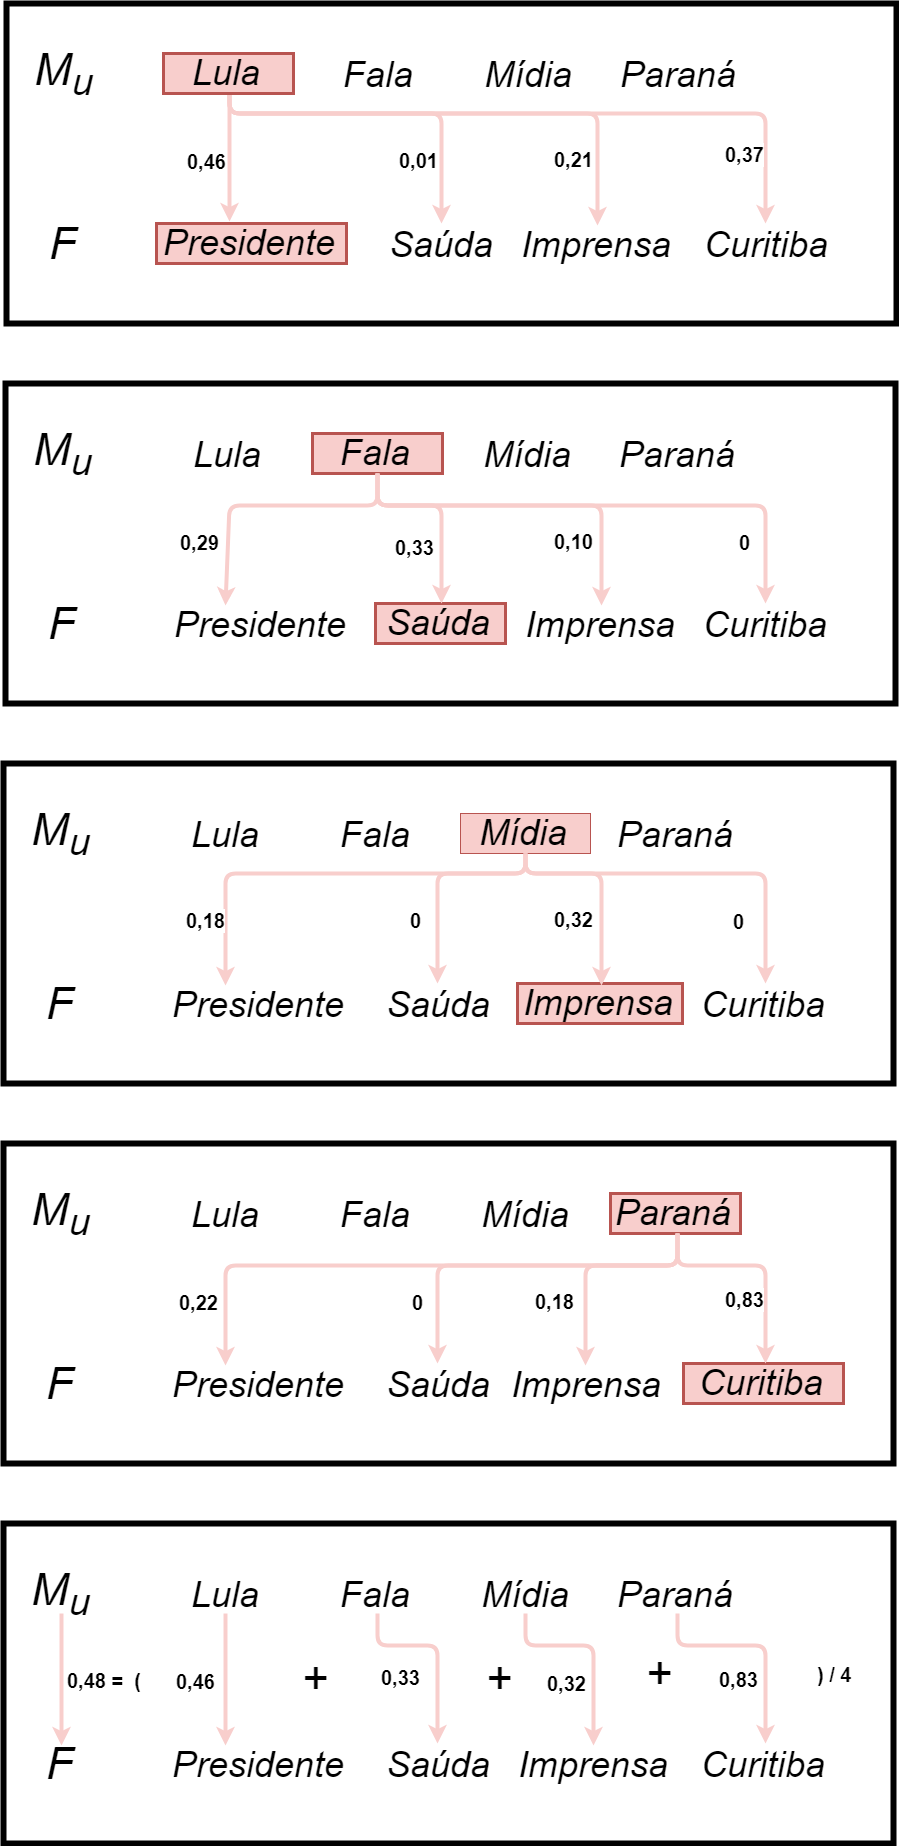
\includegraphics[scale=0.32]{imagens/rlws_ex.png}
	\caption{Imagem que exemplifica o fluxo da recomendação.}
	\label{fig:rlws_ex}
\end{figure}

\section{Estrutura de Cache para Recomendação}
\label{sec:cache}

É importante ressaltar que para este projeto foi desenvolvido um sistema de \textit{cache} para o cálculo da similaridade de recomendação dos filmes, dividido-se em duas camadas:

\begin{itemize}
	\item{\textbf{Cache remoto com banco de dados}: Para calcular a similaridade entre dois tokens quaisquer, o sistema utiliza uma Equação (\ref{eq:rlws}) de similaridade que tira proveito do serviço da DBPedia. Na equação, conforme abordado em \ref{ssec:sim_rec} realiza-se a contagem de links diretos e indiretos dos recursos. Essa contagem posteriormente é armazenada no banco de dados para uma consulta mais ágil.}
	\item{\textbf{Cache local, em memória}: A cada comparação realizada é verificado inicialmente se a mesma está presente no cache remoto, evitando consultas desnecessárias ao DBPedia. Após a verificação, a comparação é armazenada num cache local em memória de execução (\ac{RAM}). O objetivo é que durante o cálculo da recomendação de um usuário não seja necessário realizar a todo instante consultas ao banco, visto o volume de comparações, já que cada palavra dos termos do usuário é comparada com todas as palavras dos filmes. O processo de realizar tais consultas ao banco no momento da comparação prejudica o desempenho da aplicação. Assim, optou-se por utilizar a estrutura de \textit{cache} em memória fornecida pelo \textit{framework} Spring\footnote{https://spring.io}. Após um determinado número de comparações o sistema verifica quais delas precisam ser persistidas, salvando-as em sequência e posteriormente liberando o cache em memória.}
\end{itemize}

Com esse sistema minimiza-se o tráfego de dados entre a aplicação, o DBPedia e o banco de dados durante a comparação de filmes, acelerando o processo, além de ter um bom balanço de desempenho entre o cache remoto e cache local.

\section{Tecnologias}

Para o desenvolvimento do sistema foram escolhidas algumas tecnologias para arquitetura software, como linguagens de programação, \textit{framework} \ac{MVC}, processamento e banco dados, entre outras. A seguir serão apresentadas as tecnologias utilizadas.

\subsection{JAVA}

JAVA\footnote{https://www.java.com} é uma linguagem de programação de propósito genérico, desenvolvida originalmente por James Gosling na Sun Microsystems\footnote{ https://www.oracle.com/br/sun/index.html} em 1995. Atualmente a linguagem foi comprada pela Oracle Corporation\footnote{https://www.oracle.com}. As características em destaque da linguagem estão no fato de ser baseada em classes e orientada a objetos. A \ac{OOP} é um paradigma de programação que abstrai conceitos em objetos, que podem conter dados, campos e comportamentos nomeados de \textit{methods} \citep{Lewis2000}.

Outra caraterística importante da linguagem trata-se da filosofia apresentada pelos desenvolvedores de “escreva uma vez, rode em qualquer lugar”. A filosofia trata-se da linguagem ser compilada por uma \ac{VM} possibilitando escrever um mesmo pedaço de código que possa ser portado para outra plataforma sem necessidade de alterá-lo, uma vez que cada \ac{VM} implementa as especificidades da nova plataforma abstraindo o acesso ao \ac{SO}.

A linguagem JAVA é usada em diversos sistemas e plataformas, com inúmeros propósitos, desde aplicações \textit{desktop}, pesquisa científica, desenvolvimento Web entre outros propósitos.

\subsection{Spring Boot}

Spring Boot\footnote{https://projects.spring.io/spring-boot/} é um projeto da Pivotal Software\footnote{https://pivotal.io} para facilitar o processo de configuração e publicação de aplicações e serviços providos pelo Spring\footnote{https://spring.io}, com baixo esforço e configuração. O \textit{Spring} é um framework \textit{open source}\footnote{Modelo de desenvolvimento que promove um licenciamento livre para o design ou esquematização de um produto} que provê um compreensivo conjunto de modelos de configuração para aplicações JAVA. O elemento principal do \textit{Spring} é prover infraestrutura para aplicações oferecendo os seguintes principais recursos:

\begin{itemize}
	\item{\textbf{Inversão de Controle}: \ac{IOC}, também conhecido como \textit{dependency injection} é um princípio em que as “dependências” devem ser supridas, injetadas por outro objeto. As dependências são objetos que serão usados como “serviços” para acessar suas funcionalidades, dentro dos \textit{containers} de \ac{IOC}. A injeção é a passagem da dependência para um objeto (o cliente) \citep{DependencyInjection2006}. O termo “inversão de controle” origina-se do fato que a criação de valores de classes externas ao objeto não deve ser realizada pelo próprio objeto mas, sim pelos \textit{containers} de \ac{IOC}.}

	\item{\textbf{Acesso a dados}: O framework possui diversas bibliotecas para o acesso a dados, tanto para bancos relacionais como não relacionais. Também é oferecido um sistema \ac{ORM} que trata-se de uma técnica para traduzir o formato de dados de um banco relacional para \ac{OOP}, facilitando sua manipulação.}

	\item{\textbf{Arquitetura MVC}: Fornece todo suporte para customizar e criar uma arquitetura \ac{MVC}.}
\end{itemize}

\subsection{HTML, CSS, Javascript}

O HTML\footnote{https://www.w3.org/html}, \ac{CSS}\footnote{https://www.w3.org/Style/CSS/} e JavaScript forma a principal pilha de tecnologias utilizadas na Web. O HTML é uma linguagem de marcação mantida pela \ac{W3C} para criação de páginas, originalmente desenvolvida por Tim-Berners-Lee \citep{Raggett1998}. O objetivo é a fácil construção e publicação de conteúdo no ambiente Web e consequentemente na \ac{WWW}. No \textit{Spring Boot} as páginas HTML podem ser escritas utilizando algum dos mecanismos de \textit{templates}, como o \textit{thymeleaf}. Uma das vantagens da utilização desses mecanismos é a herança de visualizações, assim como facilidade de interligar em manipular os dados passados pela camada do \textit{controller} no \ac{MVC}.

O \ac{CSS} é uma linguagem para criar regras de estilização das páginas \ac{HTML}. O CSS cria ou altera um formato de apresentação (tamanho, cores, margens etc) de algum elemento do HTML, como blocos, parágrafos, imagens entre outros. Quanto ao JavaScript é uma linguagem de programação originalmente criada por Brendan Eich na Netscape Communications\footnote{ http://isp.netscape.com}. A linguagem é utilizada para controlar o comportamento de páginas HTML, oferecendo dinamicidade, podendo alterar elementos da página em tempo real.

\subsection{MySQL}

O MySQL\footnote{https://www.mysql.com} trata-se de um \ac{SGBD} que utiliza a linguagem \ac{SQL} para manipulação de dados guardados em um sistema de arquivos \citep{MySQLSGBD}. Originalmente desenvolvido por Michael Widenius em 1994, o seu foco é para o desenvolvimento de aplicações Web, embora tenha se popularizado para a maioria das plataformas existentes \citep{MySQLDevelopers}. Foi o banco de dados escolhido para a persistência de dados da aplicação, além de ser de fácil integração com o \textit{framework} \textit{Spring Boot}.

\subsection{Apache Jena}

Apache Jena\footnote{https://jena.apache.org} é um \textit{framework} \textit{open source} para Web Semântica, escrito na linguagem Java. A biblioteca provê uma \ac{API} que facilita a extração e criação de dados nos grafos do \ac{RDF}, além de oferecer suporte para a linguagem de consulta \ac{SPARQL}. O objetivo da escolha dessa tecnologia para o projeto, é para facilitar a busca e navegação pelo grafo de entidades (\textit{resources}) no sistema da DBPedia\footnote{http://wiki.dbpedia.org} utilizando \ac{SPARQL}. Após o \ac{SR} extrair entidades das descrições do filme, essas serão buscadas no serviço da Web Semântica estendendo o conhecimento do recurso.

\subsection{Apache OpenNLP}
\label{ssec:open_nlp}

Apache OpenNLP\footnote{https://opennlp.apache.org} é um \textit{framework} \textit{open source} de aprendizado de máquina que é usado para processamento de \ac{NLP}. A biblioteca provê uma \ac{API} com serviços para geração de \textit{tokens}, sentenças, segmentação, reconhecimento de partes da fala, extração de entidade de nome, geração de \textit{chunks} (pedaços), entre outras tarefas do \ac{NLP}.

No projeto essa tecnologia será utilizada para o \ac{NER} e extração de partes gramaticais presentes na descrição do filme, assim como a geração dos \textit{tokens}. O objetivo é que com essa biblioteca seja possível gerar \textit{tokens} com entidades encontradas, de nomes localizações, como também partes do texto de nomes próprios, substantivos e adjetivos.

\subsection{Apache Lucene}

Apache Lucene\footnote{https://lucene.apache.org} é um \textit{framework} \textit{open source} para sistemas de recuperação de informação e recomendação. O projeto oferece dois principais recursos: indexação e pesquisa de texto. Lucene é muito reconhecido por sua utilidade na implementação em mecanismos de buscas na Internet \citep{McCandless2010}. O projeto também é muito utilizado em sistemas de recomendação com implementação de diversos algoritmos para calcular a similaridade de documentos.
No projeto essa tecnologia será utilizada para tirar proveito dos algoritmos de similaridade, como o \textit{cossine similarity} (ver \ref{eq:cosine_sim}), possibilitando realizar comparações com as métricas propostas no trabalho.

\section{Sumário}

Neste capítulo foram apresentadas as funcionalidades para a proposta do sistema de recomendação, assim como as tecnologias empregadas. Também foram abordadas as etapas do ciclo de vida da aplicação, demonstrando o modelo de dados, assim como a etapa de preparação para recomendação. Por fim foi elaborada a proposta de um novo método de similaridade semântica, mostrando suas características e equações, além dos algoritmos para geração das recomendações. No próximo capítulo serão apresentados os resultados obtidos com novo método elaborado, junto técnicas para sua obtenção, assim como a comparação com outros modelos.
